% Boxes of text with inline math, in nodes of a set text width, saved in
% a box: their size stays known, so the picture's anchors do, and the
% color code after it runs once.
\documentclass{article}
\usepackage{tikz}
\usetikzlibrary{positioning}
\newcommand{\entry}[2]{%
  \node[below=1mm of #1, text width=2cm, rounded corners, draw=blue!20, fill=blue!10] (#2)
    {\small\begin{obeylines}$\dots$ and $x_1$\end{obeylines}};}
\begin{document}
\newsavebox{\sketch}
\sbox{\sketch}{\parbox{0.2\textwidth}{%
  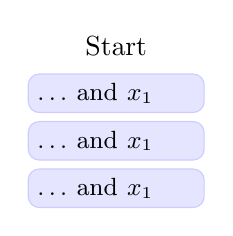
\begin{tikzpicture}
    \node (a) {Start};
    \entry{a}{b}
    \entry{b}{c}
    \entry{c}{d}
  \end{tikzpicture}}}
\colorlet{mixed}{gray!50!blue}
\begin{tikzpicture}
  \node[fill=mixed] (s) {\usebox{\sketch}};
  \node[right=1cm of s, draw] {$\langle a, b \rangle$};
\end{tikzpicture}
\gdef\SatexReachedEnd{}
\end{document}
